\documentclass[oneside,11pt]{article}

\usepackage{amsmath,graphicx,rotating}

\setlength{\oddsidemargin}{0in}
\setlength{\textwidth}{6.5in}
\setlength{\topmargin}{-.5 in}
\setlength{\textheight}{8.75in}
\begin{document}

\begin{center}
{\bf Worksheet 6 --- Math 126 --- Summer 2010}
\end{center}

The purpose of this worksheet is to give you some practice doing double integrals. They will definitely not be easy. Good luck!
\begin{enumerate}
\item Find the volume under the surface $z=2x+y^2$ and above the region in the first quadrant of the $xy$ plane that is bounded by $y=x^2$ and $y=x^3$.

\vfill 
\hfill \begin{turn}{180}{\footnotesize Answer: $4/35$}\end{turn}

\newpage
\item
\begin{minipage}[t]{4.5in}
Let $R$ be the following shaded region to the right. Compute the following integral: [Hint: you will have to split the region into at least two peices]
$$\iint_R 2x \, dA$$
\end{minipage}
\begin{minipage}[t]{2in}\vspace{-10pt}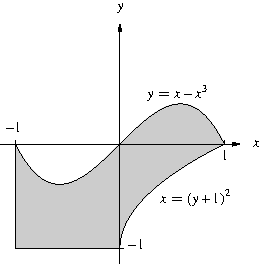
\includegraphics{ws6-region.pdf}\end{minipage}

\vfill
\hfill \begin{turn}{180}{\footnotesize Answer: $-4/15$}\end{turn}
\newpage
\item Find the volume of the space bounded by the two cylinders $x^2+y^2=1$ and $y^2+z^2=1$. [Hints:\\

\vspace{-22pt}
{\begin{enumerate}\footnotesize
\item Imagine the second cylinder as a tunnel going over the top of you. What is the equation for the height of the tunnel?
\item Integrate the height of the tunnel over the region $x^2+y^2=1$ to get the volume between the tunnel and above the ``ground''. Since the region is symmetric, we multiply that answer by 2 to get the final answer.
\item You have the choice to integrate with respect to $y$ and then $x$ or $x$ first then $y$. One of these makes the integral really difficult, so do it the easy way.]
\end{enumerate}}

\begin{center}
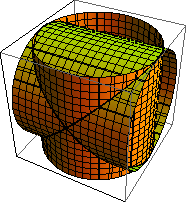
\includegraphics[width=.3\textwidth]{ws6-intersect1.png}
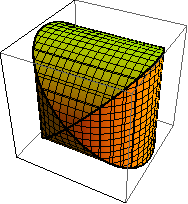
\includegraphics[width=.3\textwidth]{ws6-intersect2.png}
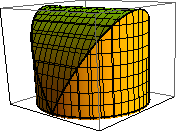
\includegraphics[width=.3\textwidth]{ws6-intersect3.png}\\
\hspace{.2in}The two cylinders\hspace{.85in} The intersection \hfill The top half of the intersection
\end{center}

\vfill 

\hfill \begin{turn}{180}{\footnotesize Answer: rhymes with ``mixed green nerds''}\end{turn}
\end{enumerate}
\end{document}

